% ============================================================================
%  HAT-MedMNIST  --  project presentation
%  Theme: Flux (installed globally in TEXMFHOME/tex/latex/flux-beamer)
%  Build: pdflatex presentation.tex   (run twice for the frame numbers / TOC)
%
%  Organisation: three equal-length parts (shared talk), 6 slides each --
%    1. "Motivation, Objectives & Plan"        -- Project Manager (Stefano Verrilli)
%    2. "System Architecture & MVP"            -- Technical Manager (Giuseppe Todisco)
%    3. "Prior Art, Governance & Validation"   -- Reviewer (Mohammad Dolatabadi)
%  Section titles name the TOPIC each speaker covers, not the presenter split
%  (attribution stays on the title page / institute line). Sections appear in
%  the outline only; the Flux theme adds no divider slides.
%  Slide-to-role assignment follows the proposal's responsibility table: TR
%  owns architecture/agent-build content (incl. the Prior-Art Scout's design),
%  REV owns audit/governance/acceptance content (incl. leakage-safety audit),
%  PM owns scope/schedule/risk content.
% ============================================================================
\documentclass[10pt,aspectratio=169]{beamer}

% Flux is installed globally, so a plain \usetheme is enough.
% Styles available: asphalt | blue | red | green | gray
\usetheme[style=green]{flux}

\usepackage[utf8]{inputenc}
\usepackage[T1]{fontenc}
\usepackage{booktabs}
\usepackage{array}
\usepackage{graphicx}
\usepackage{tikz}
\usetikzlibrary{arrows.meta,positioning,shadows,backgrounds}

% palette echoing the Flux "green" style, for the proposal diagram
\definecolor{fxgreen}{HTML}{5E7A29}
\definecolor{fxlight}{HTML}{E7ECD8}
\definecolor{fxgrey}{HTML}{E9E9E9}
\definecolor{fxorange}{HTML}{C7791F}
\tikzset{
  box/.style={rounded corners=2pt, align=center, text width=2.35cm,
              minimum height=1.05cm, font=\small, inner sep=3pt},
  det/.style={box, fill=fxgrey},
  hyb/.style={box, fill=fxlight, draw=fxgreen, thick},
  gov/.style={box, fill=fxorange!12, draw=fxorange, dashed, thick},
  arr/.style={-{Stealth[length=2mm]}, thick, draw=fxgreen},
}

% -------- title metadata -----------------------------------------------------
\title{HAT-MedMNIST}
\subtitle{A hybrid agentic training framework for MedMNIST}
% keep the subtitle within the slide width
\setbeamerfont{subtitle}{size=\large,series=\bfseries}
\author{Giuseppe Todisco \and Stefano Verrilli \and Mohammad Dolatabadi}
\institute{Technical Responsible \enspace$\cdot$\enspace Project Manager \enspace$\cdot$\enspace Reviewer
  \\[0.4em] Agentic AI / medical-image benchmarks}
\date{\today}

\begin{document}

% NOTE: with the Flux theme \titlepage already opens its own frame,
% so it must NOT be wrapped in \begin{frame}...\end{frame}.
\titlepage

% ---------------------------------------------------------------------------
\begin{frame}{Outline}
  \tableofcontents
\end{frame}

% ===========================================================================
\section{Motivation, Objectives \& Plan}
% ===========================================================================
\begin{frame}{What it is}
  A \textbf{modular, hybrid agentic framework} for training neural networks on
  MedMNIST.
  \vspace{0.6em}
  \begin{itemize}
    \item Role-specialised agents own \textbf{one duty each}.
    \item They interact \textbf{only through versioned artefacts}.
    \item An independent reviewer agent \textbf{audits every stage and can veto}.
  \end{itemize}
  \vspace{0.6em}
  \begin{block}{The contribution}
    The orchestration is the contribution --- \textbf{not} the classifier.
  \end{block}
\end{frame}

\begin{frame}{Why it matters}
  \begin{columns}[T]
    \begin{column}{0.5\textwidth}
      \textbf{Conventional pipelines}
      \begin{itemize}
        \item Tightly coupled.
        \item Hard to reproduce and audit.
      \end{itemize}
      \vspace{0.8em}
      \textbf{Typical LLM-agent frameworks}
      \begin{itemize}
        \item Non-determinism everywhere.
        \item Locked to one proprietary model.
      \end{itemize}
    \end{column}
    \begin{column}{0.5\textwidth}
      \begin{block}{HAT-MedMNIST}
        \begin{itemize}
          \item Roles \emph{plus} explicit contracts.
          \item Non-determinism confined to declared decisions.
          \item Every choice is traceable.
          \item An independent automated reviewer.
        \end{itemize}
      \end{block}
    \end{column}
  \end{columns}
\end{frame}

\begin{frame}{Objectives}
  \begin{itemize}
    \item Cohesive, weakly-coupled agents that talk only via typed artefacts.
    \item A \textbf{representation-architect} agent that reasons about the best input.
    \item A \textbf{hybrid reasoning seam}: open models with heuristic fallback.
    \item \textbf{Ambiguity handling} and leakage-safe data splits.
    \item \textbf{Abstention} on the ``no confident finding'' case.
    \item An integrated MVP demonstrated at \textbf{TRL 7}.
  \end{itemize}
\end{frame}

\begin{frame}{Work packages}
  \normalsize
  \renewcommand{\arraystretch}{1.6}
  \setlength{\tabcolsep}{18pt}
  \begin{center}
  \begin{tabular}{@{}ll@{}}
    \toprule
    \textbf{WP} & \textbf{Focus} \\
    \midrule
    WP1 & Requirements \& architecture \\
    WP2 & Data understanding, representation \& prior-art scouting \\
    WP3 & Hybrid orchestration \& prior-art-informed model design \\
    WP4 & Evaluation, enrichment \& comparison \\
    WP5 & MVP integration \& validation \\
    WP6 & Consistency \& anomaly governance (cross-cutting) \\
    \bottomrule
  \end{tabular}
  \end{center}
\end{frame}

\begin{frame}{Indicative 12-month plan}
  \normalsize
  \renewcommand{\arraystretch}{1.5}
  \setlength{\tabcolsep}{7pt}
  \begin{center}
  \begin{tabular}{@{}l*{12}{c}@{}}
    \toprule
    \textbf{WP\,/\,Month} & 1&2&3&4&5&6&7&8&9&10&11&12\\
    \midrule
    WP1 & \textbullet&\textbullet& & & & & & & & & & \\
    WP2 & &\textbullet&\textbullet&\textbullet& & & & & & & & \\
    WP3 & & &\textbullet&\textbullet&\textbullet&\textbullet&\textbullet& & & & & \\
    WP4 & & & & &\textbullet&\textbullet&\textbullet&\textbullet&\textbullet& & & \\
    WP5 & & & & & & & &\textbullet&\textbullet&\textbullet&\textbullet&\textbullet\\
    WP6 & &\textbullet&\textbullet&\textbullet&\textbullet&\textbullet&\textbullet&\textbullet&\textbullet&\textbullet&\textbullet&\textbullet\\
    \bottomrule
  \end{tabular}
  \end{center}
  \vspace{0.4em}
  {\footnotesize WP6 is cross-cutting across the whole timeline.}
\end{frame}

\begin{frame}{Risk plan}
  \small
  \renewcommand{\arraystretch}{1.3}
  \setlength{\tabcolsep}{5pt}
  \begin{center}
  \begin{tabular}{@{}lp{1.9cm}p{4.3cm}@{}}
    \toprule
    \textbf{Risk} & \textbf{Impact\,/\,\allowbreak Prob.} & \textbf{Mitigation} \\
    \midrule
    Data leakage / invalid split    & High / Med & Train-only stats, seeded splits, reviewer gate before training \\
    Non-deterministic LLM reasoning & Med / Med  & Temperature 0, heuristic fallback, logged provenance \\
    Agent contract failure          & High / Med & Typed artefact contracts, orchestrator veto, fault-injection tests \\
    Performance below baseline      & High / Med & Baseline-first strategy, ablations, documented negative results \\
    Vendor lock-in                  & Med / Low  & Open-model seam, no proprietary dependency \\
    \bottomrule
  \end{tabular}
  \end{center}
\end{frame}

% ===========================================================================
\section{System Architecture \& MVP}
% ===========================================================================
\begin{frame}{The Blackboard architecture}
  \vfill
  \centering
  \resizebox{0.94\textwidth}{!}{% Shared HAT-MedMNIST architecture diagram (clean "bars + row of boxes" layout,
% matching docs/architecture.png, with the Prior-Art Scout added).
% \input this inside \resizebox{\textwidth}{!}{...}. Requires in the preamble:
%   \usepackage{tikz}\usetikzlibrary{arrows.meta,positioning,shadows,backgrounds}
\definecolor{navy}{HTML}{16233A}
\definecolor{gfill}{HTML}{EEF1F5}
\definecolor{gline}{HTML}{C4CCD8}
\definecolor{bfill}{HTML}{DCEBFB}
\definecolor{bline}{HTML}{4C86D6}
\definecolor{oline}{HTML}{E8792E}
\definecolor{ofill}{HTML}{FDF3EA}
\definecolor{ink}{HTML}{1B2430}
\definecolor{rfill}{HTML}{ECE4FB}
\definecolor{rline}{HTML}{7C5CBF}
\begin{tikzpicture}[
  font=\sffamily,
  bar/.style={rectangle, rounded corners=2pt, fill=navy, text=white,
              minimum height=0.8cm, align=center, inner sep=4pt},
  box/.style={rectangle, rounded corners=3pt, minimum width=1.9cm,
              minimum height=1.9cm, align=center, inner sep=2pt,
              text width=1.7cm, font=\scriptsize, text=ink, line width=0.9pt,
              drop shadow={shadow xshift=1pt, shadow yshift=-1pt, opacity=0.12}},
  det/.style={box, fill=gfill, draw=gline},
  hyb/.style={box, fill=bfill, draw=bline},
  down/.style={-{Stealth[length=2.4mm]}, draw=navy!75, line width=0.9pt},
  gov/.style={-{Stealth[length=2.4mm]}, draw=oline, line width=0.9pt, dashed},
]
\def\cA{1.45}\def\cB{3.61}\def\cC{5.77}\def\cD{7.93}\def\cE{10.09}%
\def\cF{12.25}\def\cG{14.41}\def\cH{16.57}\def\cI{18.73}%
\def\barL{0.5}\def\barW{19.18}
% Symmetric bounding box centred on the bars (bars span x=0.5..19.68, centre 10.09),
% so the left-hand "veto / stop" label does not push the figure off-centre.
\useasboundingbox (-0.05,1.55) rectangle (20.23,11.85);

\node[anchor=west, text=ink, font=\sffamily\bfseries\Large] at (\barL,11.35)
  {Hybrid Agentic MedMNIST \textemdash\ architecture};
\node[anchor=west, text=ink!60, font=\sffamily\small] at (\barL,10.78)
  {Maximum cohesion, minimum coupling \textperiodcentered\ agents share only versioned artefacts};

\node[bar, anchor=south west, minimum width=\barW cm, font=\bfseries] (orch)
  at (\barL,9.8) {Orchestrator \textemdash\ sequencing \& veto handling (no ML / no domain logic)};

\node[det, anchor=south] at (\cA,6.9) {\textbf{1 \textperiodcentered\ Ingestion}\\[2pt]{\tiny WP2}};
\node[hyb, anchor=south] at (\cB,6.9) {\textbf{2 \textperiodcentered\ Profiling / Ambiguity}\\[2pt]{\tiny hybrid \textperiodcentered\ WP2}};
\node[hyb, anchor=south] at (\cC,6.9) {\textbf{Prior-Art Scout}\\[2pt]{\tiny hybrid \textperiodcentered\ WP2}};
\node[hyb, anchor=south] at (\cD,6.9) {\textbf{3 \textperiodcentered\ Preproc / Representation}\\[2pt]{\tiny hybrid \textperiodcentered\ WP2}};
\node[hyb, anchor=south] at (\cE,6.9) {\textbf{4 \textperiodcentered\ Experiment Design}\\[2pt]{\tiny hybrid \textperiodcentered\ WP3}};
\node[det, anchor=south] at (\cF,6.9) {\textbf{5 \textperiodcentered\ Training}\\[2pt]{\tiny WP3}};
\node[det, anchor=south] at (\cG,6.9) {\textbf{6 \textperiodcentered\ Evaluation}\\[2pt]{\tiny WP4}};
\node[det, anchor=south] at (\cH,6.9) {\textbf{7 \textperiodcentered\ Abstention / OOD}\\[2pt]{\tiny WP5}};
\node[det, anchor=south] at (\cI,6.9) {\textbf{8 \textperiodcentered\ Reporting}\\[2pt]{\tiny WP5}};

% ---- research-capabilities group (behind the three research / design agents) --
\begin{scope}[on background layer]
  \draw[rline, rounded corners=7pt, line width=1pt, fill=rfill]
    (4.63,6.64) rectangle (11.23,9.00);
\end{scope}

\node[bar, anchor=south west, minimum width=\barW cm, font=\bfseries] (bb)
  at (\barL,5.0) {Blackboard \textemdash\ versioned, typed artefacts (the interfaces) + decision / audit log};

\node[rectangle, rounded corners=3pt, draw=oline, dashed, fill=ofill, line width=1pt,
      text=oline, anchor=south west, minimum width=\barW cm, minimum height=0.95cm,
      align=center, font=\bfseries] (rev) at (\barL,3.1)
  {Reviewer / Consistency / Anomaly agent (WP6) \textemdash\ audits every stage \textperiodcentered\ can veto promotion};

\foreach \x in {\cA,\cB,\cC,\cD,\cE,\cF,\cG,\cH,\cI}{
  \draw[down] (\x,9.8) -- (\x,8.82);
  \draw[down] (\x,6.88) -- (\x,5.82);
}

\draw[gov] (\cE,4.05) -- (\cE,4.98);
\draw[gov] (0.30,3.55) -- (0.30,10.2) -- (\barL,10.2);
\node[text=oline, font=\sffamily\scriptsize, rotate=90, anchor=south] at (0.15,6.6) {veto / stop};

\def\ly{2.0}
\node[det, minimum width=0.5cm, minimum height=0.42cm, text width=0.4cm, anchor=west] at (\barL,\ly){};
\node[anchor=west, font=\sffamily\footnotesize, text=ink] at (1.05,\ly) {deterministic};
\node[hyb, minimum width=0.5cm, minimum height=0.42cm, text width=0.4cm, anchor=west] at (3.6,\ly){};
\node[anchor=west, font=\sffamily\footnotesize, text=ink] at (4.15,\ly) {hybrid (open-model + fallback)};
\node[rectangle, rounded corners=3pt, draw=rline, fill=rfill, minimum width=0.5cm, minimum height=0.42cm, anchor=west] at (9.2,\ly){};
\node[anchor=west, font=\sffamily\footnotesize, text=ink] at (9.75,\ly) {research \& design agents};
\node[rectangle, rounded corners=2pt, draw=oline, dashed, fill=ofill, minimum width=0.5cm, minimum height=0.42cm, anchor=west] at (14.0,\ly){};
\node[anchor=west, font=\sffamily\footnotesize, text=ink] at (14.55,\ly) {cross-cutting governance};
\end{tikzpicture}
}
  \vfill
\end{frame}

\begin{frame}{Cohesion \& coupling}
  \begin{itemize}
    \item \textbf{No agent calls another.}
    \item They share only versioned artefacts on a \textbf{Blackboard}.
    \item A stateless \textbf{Orchestrator} sequences them.
  \end{itemize}
  \vspace{0.6em}
  \begin{block}{The claim, made testable}
    Any agent can be replaced or upgraded without touching another ---
    \textbf{zero direct inter-agent calls}.
  \end{block}
\end{frame}

\begin{frame}{The agents}
  \small
  \renewcommand{\arraystretch}{1.25}
  \setlength{\tabcolsep}{13pt}
  \begin{center}
  \begin{tabular}{@{}lll@{}}
    \toprule
    \textbf{Agent} & \textbf{Duty} & \textbf{Kind} \\
    \midrule
    Orchestrator                 & sequencing, veto handling      & deterministic \\
    Ingestion                    & load MedMNIST                  & deterministic \\
    Profiling / Ambiguity        & profile data, flag ambiguity   & \textbf{hybrid} \\
    Prior-Art Scout              & search literature, propose ideas & \textbf{hybrid} \\
    Preprocessing                & architect the representation   & \textbf{hybrid} \\
    Experiment Design            & pick the configuration         & \textbf{hybrid} \\
    Training                     & train the selected model            & deterministic \\
    Evaluation                   & test metrics                   & deterministic \\
    Abstention / OOD             & refuse when unconfident        & deterministic \\
    Reporting                    & assemble the dossier           & deterministic \\
    Reviewer (WP6)               & consistency / anomaly, veto    & \textbf{hybrid} \\
    \bottomrule
  \end{tabular}
  \end{center}
\end{frame}

\begin{frame}{The Prior-Art Scout}
  A hybrid component of the pipeline: it reads the literature and feeds
  \textbf{cited ideas} into representation (step 3) and architecture (step 4).
  \vspace{0.2em}
  \begin{center}
  \resizebox{0.70\textwidth}{!}{%
  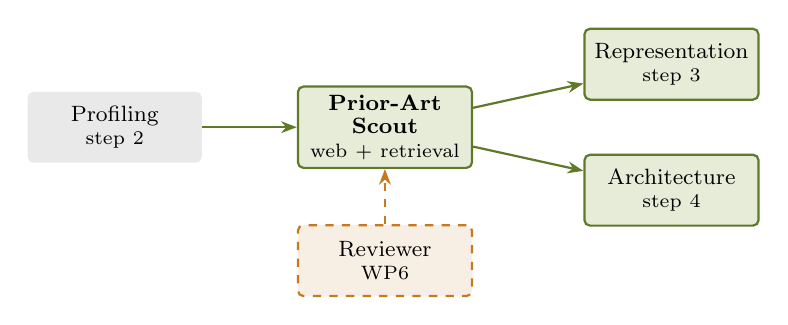
\begin{tikzpicture}[
    box/.append style={text width=2.0cm, minimum height=0.9cm, font=\footnotesize}]
    \node[det]                                  (prof)  {Profiling\\[-1pt]{\scriptsize step 2}};
    \node[hyb, right=12mm of prof]              (scout) {\textbf{Prior-Art}\\[-1pt]\textbf{Scout}\\[-1pt]{\scriptsize web + retrieval}};
    \node[hyb, right=14mm of scout, yshift=8mm] (rep)   {Representation\\[-1pt]{\scriptsize step 3}};
    \node[hyb, right=14mm of scout, yshift=-8mm](arch)  {Architecture\\[-1pt]{\scriptsize step 4}};
    \node[gov, below=7mm of scout]              (rev)   {Reviewer\\[-1pt]{\scriptsize WP6}};
    \draw[arr] (prof)  -- (scout);
    \draw[arr] (scout) -- (rep);
    \draw[arr] (scout) -- (arch);
    \draw[arr, draw=fxorange, dashed] (rev) -- (scout);
  \end{tikzpicture}}
  \end{center}
  \vspace{0.8em}
  {\footnotesize It \emph{advises} the hybrid decisions --- it never trains,
  selects, or calls another agent.}
\end{frame}

\begin{frame}{The hybrid approach}
  \begin{columns}[T]
    \begin{column}{0.5\textwidth}
      \textbf{Deterministic execution}
      \begin{itemize}
        \item data, splits, training, metrics, ranking.
      \end{itemize}
      \vspace{0.6em}
      \textbf{Open-model reasoning, only at:}
      \begin{itemize}
        \item ambiguity assessment,
        \item representation design,
        \item configuration choice,
        \item consistency review.
      \end{itemize}
    \end{column}
    \begin{column}{0.5\textwidth}
      \begin{block}{No vendor lock-in}
        Plug in a local open model. With none, it falls back to heuristics and
        still runs offline and reproducibly.
      \end{block}
      \vspace{0.4em}
      \begin{block}{Reproducible reasoning}
        Every decision records its source; identical seeds and configs replay
        the run.
      \end{block}
    \end{column}
  \end{columns}
\end{frame}

\begin{frame}{The MVP}
  \begin{itemize}
    \item Runs end-to-end on \textbf{PathMNIST} (nine-class histology).
    \item Preserves the \textbf{official split}; the test set is a different clinical centre.
    \item Agents \textbf{search and train} bounded architectures automatically.
    \item Compared against a \textbf{conventional baseline} on the same data and seeds.
  \end{itemize}
\end{frame}

% ===========================================================================
\section{Prior Art, Governance \& Validation}
% ===========================================================================
\begin{frame}{Leakage-safe by design}
  \begin{itemize}
    \item The search loop \textbf{never sees test metrics}.
    \item Selection is driven by \textbf{validation only}.
    \item The winner is frozen, then evaluated on test \textbf{once}.
    \item Repeated seeds quantify run-to-run variance.
  \end{itemize}
  \vspace{0.6em}
  \begin{block}{Independent audit}
    A data-quality and leakage audit must pass \textbf{before} any training
    begins.
  \end{block}
\end{frame}

\begin{frame}{From literature to decisions}
  Two levels, at very different cost:
  \begin{itemize}
    \item \textbf{Advise within bounds} --- rank \& justify existing options with
          evidence. Cheap, safe, immediate.
    \item \textbf{Propose new options} --- outside the current set; promoted
          through a gate before anything runs.
  \end{itemize}
  \vspace{0.4em}
  \begin{columns}[T]
    \begin{column}{0.5\textwidth}
      \begin{block}{Representation (step 3)}
        New label-preserving augmentations: validated, then whitelisted ---
        \textbf{semi-automatic}.
      \end{block}
    \end{column}
    \begin{column}{0.5\textwidth}
      \begin{block}{Architecture (step 4)}
        A new family stays a \textbf{reviewed spec} --- implemented as a registry
        entry, then runnable.
      \end{block}
    \end{column}
  \end{columns}
\end{frame}

\begin{frame}{Reproducible \& governed}
  \begin{columns}[T]
    \begin{column}{0.5\textwidth}
      \textbf{Reproducible by design}
      \begin{itemize}
        \item Snapshot + checksum every source.
        \item A rerun replays the cache.
        \item Temperature 0; heuristic fallback when offline.
      \end{itemize}
    \end{column}
    \begin{column}{0.5\textwidth}
      \textbf{Governed (WP6)}
      \begin{itemize}
        \item The Reviewer verifies every citation resolves.
        \item Claims must be backed by a source.
        \item It can \textbf{veto} the brief.
      \end{itemize}
    \end{column}
  \end{columns}
  \vspace{0.6em}
  \begin{block}{Measured}
    100\% of ideas cited \enspace$\cdot$\enspace 0 hallucinated citations
    \enspace$\cdot$\enspace brief reproducible from the cache.
  \end{block}
\end{frame}

\begin{frame}{Governance as an agent (WP6)}
  \begin{itemize}
    \item An \textbf{independent reviewer} audits each stage.
    \item It can request a \textbf{retry} or \textbf{veto} promotion.
    \item It checks evidence, traceability and reproducibility.
  \end{itemize}
  \vspace{0.6em}
  \begin{block}{Measured}
    $\geq$90\% of injected inconsistencies detected \enspace$\cdot$\enspace
    100\% of decisions logged \enspace$\cdot$\enspace full run reproducible.
  \end{block}
\end{frame}

\begin{frame}{Target: TRL 7}
  \begin{block}{System prototype in a representative environment}
    An end-to-end workflow --- ingestion, representation, coordinated decisions,
    training, evaluation, abstention, auditing --- demonstrated by someone other
    than the implementer.
  \end{block}
  \vspace{0.4em}
  \begin{itemize}
    \item Research demonstrator on \textbf{benchmark data}.
    \item \textbf{No clinical claims}; uncertain cases go to human review.
  \end{itemize}
\end{frame}

\begin{frame}{Final acceptance criteria}
  \begin{itemize}
    \item All mandatory deliverables complete, versioned, and linked to requirements.
    \item KPIs measured with documented procedures and objective evidence.
    \item End-to-end hybrid workflow demonstrated, including abstention on uncertain cases.
    \item Results reproducible from stored configs, code, data references and seeds.
    \item No critical risk remains without an approved mitigation.
  \end{itemize}
  \vspace{0.6em}
  \begin{block}{Reviewer sign-off}
    Confirms coherence of the scientific advancement, industrial potential, and TRL~7 evidence.
  \end{block}
\end{frame}

% ---------------------------------------------------------------------------
\begin{frame}[plain]
  \begin{center}
    \vspace{1.2cm}
    {\usebeamerfont{title}\usebeamercolor[fg]{title}\Huge Thank you}\\[0.6cm]
    {\large Maximum cohesion, minimum coupling.}
  \end{center}
\end{frame}

\end{document}
